\chapter{有向图}

在本章中，我们重点关注两类有向图：
\begin{itemize}
\item \key{无环图}：
图中没有环，
因此没有任何节点到自身的路径\footnote{有向无环图有时被称为DAG。}。
\item \key{后继图}：
每个节点的出度为1，
因此每个节点有唯一的后继。
\end{itemize}
事实证明，在这两种情况下，
我们都可以基于图的特殊性质
设计高效的算法。

\section{拓扑排序}

\index{拓扑排序}
\index{环}

\key{拓扑排序}是图中节点的一种排列方式，
使得如果存在从节点 $a$ 到节点 $b$ 的路径，
则在排列中节点 $a$ 出现在节点 $b$ 之前。
例如，对于以下图
\begin{center}
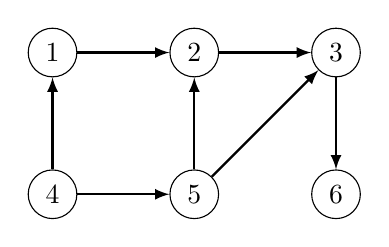
\begin{tikzpicture}[scale=0.9]
\node[draw, circle] (1) at (1,5) {$1$};
\node[draw, circle] (2) at (3,5) {$2$};
\node[draw, circle] (3) at (5,5) {$3$};
\node[draw, circle] (4) at (1,3) {$4$};
\node[draw, circle] (5) at (3,3) {$5$};
\node[draw, circle] (6) at (5,3) {$6$};

\path[draw,thick,->,>=latex] (1) -- (2);
\path[draw,thick,->,>=latex] (2) -- (3);
\path[draw,thick,->,>=latex] (4) -- (1);
\path[draw,thick,->,>=latex] (4) -- (5);
\path[draw,thick,->,>=latex] (5) -- (2);
\path[draw,thick,->,>=latex] (5) -- (3);
\path[draw,thick,->,>=latex] (3) -- (6);
\end{tikzpicture}
\end{center}
一个拓扑排序是
$[4,1,5,2,3,6]$：
\begin{center}
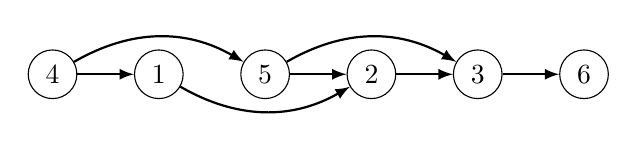
\begin{tikzpicture}[scale=0.9]
\node[draw, circle] (1) at (-6,0) {$1$};
\node[draw, circle] (2) at (-3,0) {$2$};
\node[draw, circle] (3) at (-1.5,0) {$3$};
\node[draw, circle] (4) at (-7.5,0) {$4$};
\node[draw, circle] (5) at (-4.5,0) {$5$};
\node[draw, circle] (6) at (-0,0) {$6$};

\path[draw,thick,->,>=latex] (1) edge [bend right=30] (2);
\path[draw,thick,->,>=latex] (2) -- (3);
\path[draw,thick,->,>=latex] (4) -- (1);
\path[draw,thick,->,>=latex] (4) edge [bend left=30] (5);
\path[draw,thick,->,>=latex] (5) -- (2);
\path[draw,thick,->,>=latex] (5) edge [bend left=30]  (3);
\path[draw,thick,->,>=latex] (3) -- (6);
\end{tikzpicture}
\end{center}

无环图总是存在拓扑排序。
然而，如果图中包含环，
则无法形成拓扑排序，
因为环中的任何节点都无法在排列中
出现在环中其他节点之前。
事实证明，深度优先搜索既可以用来检查有向图是否包含环，
也可以在不含环的情况下构造拓扑排序。

\subsubsection{算法}

基本思想是遍历图中的节点，
如果当前节点尚未被处理，
则从该节点开始深度优先搜索。
在搜索过程中，节点有三种可能的状态：

\begin{itemize}
\item 状态0：节点尚未被处理（白色）
\item 状态1：节点正在处理中（浅灰色）
\item 状态2：节点已被处理（深灰色）
\end{itemize}

初始时，每个节点的状态为0。
当搜索首次到达某个节点时，
其状态变为1。
最后，当该节点的所有后继
都已被处理后，其状态变为2。

如果图中包含环，我们将在搜索过程中发现这一点，
因为迟早会遇到状态为1的节点。
在这种情况下，无法构造拓扑排序。

如果图不包含环，我们可以构造拓扑排序，方法是将每个节点在其状态变为2时添加到一个列表中。
该列表的逆序即为拓扑排序。

\subsubsection{示例1}

在示例图中，搜索首先从
节点1进行到节点6：

\begin{center}
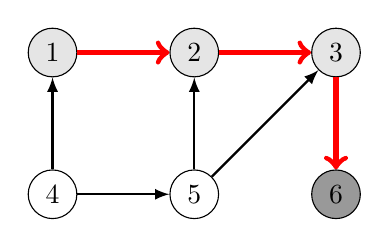
\begin{tikzpicture}[scale=0.9]
\node[draw, circle,fill=gray!20] (1) at (1,5) {$1$};
\node[draw, circle,fill=gray!20] (2) at (3,5) {$2$};
\node[draw, circle,fill=gray!20] (3) at (5,5) {$3$};
\node[draw, circle] (4) at (1,3) {$4$};
\node[draw, circle] (5) at (3,3) {$5$};
\node[draw, circle,fill=gray!80] (6) at (5,3) {$6$};

\path[draw,thick,->,>=latex] (4) -- (1);
\path[draw,thick,->,>=latex] (4) -- (5);
\path[draw,thick,->,>=latex] (5) -- (2);
\path[draw,thick,->,>=latex] (5) -- (3);
%\path[draw,thick,->,>=latex] (3) -- (6);

\path[draw=red,thick,->,line width=2pt] (1) -- (2);
\path[draw=red,thick,->,line width=2pt] (2) -- (3);
\path[draw=red,thick,->,line width=2pt] (3) -- (6);
\end{tikzpicture}
\end{center}

现在节点6已被处理，因此将其添加到列表中。
此后，节点3、2和1也被添加到列表中：

\begin{center}
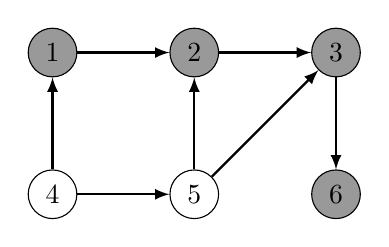
\begin{tikzpicture}[scale=0.9]
\node[draw, circle,fill=gray!80] (1) at (1,5) {$1$};
\node[draw, circle,fill=gray!80] (2) at (3,5) {$2$};
\node[draw, circle,fill=gray!80] (3) at (5,5) {$3$};
\node[draw, circle] (4) at (1,3) {$4$};
\node[draw, circle] (5) at (3,3) {$5$};
\node[draw, circle,fill=gray!80] (6) at (5,3) {$6$};

\path[draw,thick,->,>=latex] (1) -- (2);
\path[draw,thick,->,>=latex] (2) -- (3);
\path[draw,thick,->,>=latex] (4) -- (1);
\path[draw,thick,->,>=latex] (4) -- (5);
\path[draw,thick,->,>=latex] (5) -- (2);
\path[draw,thick,->,>=latex] (5) -- (3);
\path[draw,thick,->,>=latex] (3) -- (6);
\end{tikzpicture}
\end{center}

此时，列表为 $[6,3,2,1]$。
下一次搜索从节点4开始：

\begin{center}
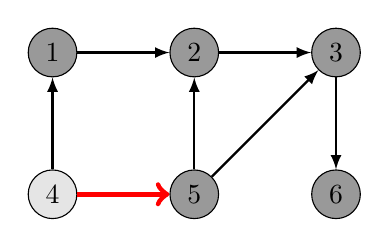
\begin{tikzpicture}[scale=0.9]
\node[draw, circle,fill=gray!80] (1) at (1,5) {$1$};
\node[draw, circle,fill=gray!80] (2) at (3,5) {$2$};
\node[draw, circle,fill=gray!80] (3) at (5,5) {$3$};
\node[draw, circle,fill=gray!20] (4) at (1,3) {$4$};
\node[draw, circle,fill=gray!80] (5) at (3,3) {$5$};
\node[draw, circle,fill=gray!80] (6) at (5,3) {$6$};

\path[draw,thick,->,>=latex] (1) -- (2);
\path[draw,thick,->,>=latex] (2) -- (3);
\path[draw,thick,->,>=latex] (4) -- (1);
%\path[draw,thick,->,>=latex] (4) -- (5);
\path[draw,thick,->,>=latex] (5) -- (2);
\path[draw,thick,->,>=latex] (5) -- (3);
\path[draw,thick,->,>=latex] (3) -- (6);

\path[draw=red,thick,->,line width=2pt] (4) -- (5);
\end{tikzpicture}
\end{center}

因此，最终列表为 $[6,3,2,1,5,4]$。
我们已处理所有节点，因此找到了拓扑排序。
拓扑排序是逆序列表
$[4,5,1,2,3,6]$：

\begin{center}
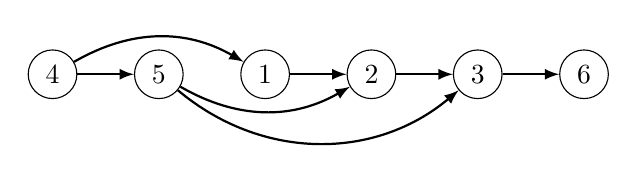
\begin{tikzpicture}[scale=0.9]
\node[draw, circle] (1) at (3,0) {$1$};
\node[draw, circle] (2) at (4.5,0) {$2$};
\node[draw, circle] (3) at (6,0) {$3$};
\node[draw, circle] (4) at (0,0) {$4$};
\node[draw, circle] (5) at (1.5,0) {$5$};
\node[draw, circle] (6) at (7.5,0) {$6$};

\path[draw,thick,->,>=latex] (1) -- (2);
\path[draw,thick,->,>=latex] (2) -- (3);
\path[draw,thick,->,>=latex] (4) edge [bend left=30] (1);
\path[draw,thick,->,>=latex] (4) -- (5);
\path[draw,thick,->,>=latex] (5) edge [bend right=30] (2);
\path[draw,thick,->,>=latex] (5) edge [bend right=40] (3);
\path[draw,thick,->,>=latex] (3) -- (6);
\end{tikzpicture}
\end{center}

注意，拓扑排序不是唯一的，
一个图可能有多种拓扑排序。

\subsubsection{示例2}

现在考虑一个无法构造拓扑排序的图，
因为该图包含环：

\begin{center}
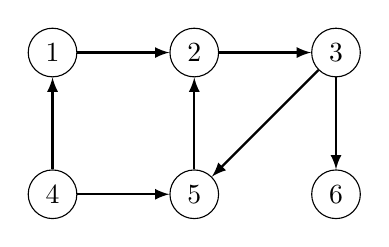
\begin{tikzpicture}[scale=0.9]
\node[draw, circle] (1) at (1,5) {$1$};
\node[draw, circle] (2) at (3,5) {$2$};
\node[draw, circle] (3) at (5,5) {$3$};
\node[draw, circle] (4) at (1,3) {$4$};
\node[draw, circle] (5) at (3,3) {$5$};
\node[draw, circle] (6) at (5,3) {$6$};

\path[draw,thick,->,>=latex] (1) -- (2);
\path[draw,thick,->,>=latex] (2) -- (3);
\path[draw,thick,->,>=latex] (4) -- (1);
\path[draw,thick,->,>=latex] (4) -- (5);
\path[draw,thick,->,>=latex] (5) -- (2);
\path[draw,thick,->,>=latex] (3) -- (5);
\path[draw,thick,->,>=latex] (3) -- (6);
\end{tikzpicture}
\end{center}
搜索过程如下：
\begin{center}
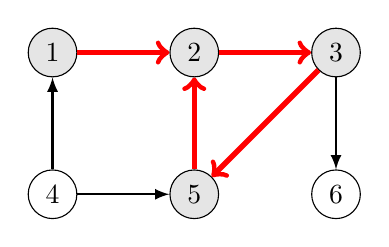
\begin{tikzpicture}[scale=0.9]
\node[draw, circle,fill=gray!20] (1) at (1,5) {$1$};
\node[draw, circle,fill=gray!20] (2) at (3,5) {$2$};
\node[draw, circle,fill=gray!20] (3) at (5,5) {$3$};
\node[draw, circle] (4) at (1,3) {$4$};
\node[draw, circle,fill=gray!20] (5) at (3,3) {$5$};
\node[draw, circle] (6) at (5,3) {$6$};

\path[draw,thick,->,>=latex] (4) -- (1);
\path[draw,thick,->,>=latex] (4) -- (5);
\path[draw,thick,->,>=latex] (3) -- (6);

\path[draw=red,thick,->,line width=2pt] (1) -- (2);
\path[draw=red,thick,->,line width=2pt] (2) -- (3);
\path[draw=red,thick,->,line width=2pt] (3) -- (5);
\path[draw=red,thick,->,line width=2pt] (5) -- (2);
\end{tikzpicture}
\end{center}
搜索到达节点2，其状态为1，
这意味着图中包含环。
在本例中，存在一个环 $2 \rightarrow 3 \rightarrow 5 \rightarrow 2$。

\section{动态规划}

如果有向图是无环的，
则可以对其应用动态规划。
例如，我们可以高效地解决以下关于从起始节点到终止节点路径的问题：

\begin{itemize}
\item 有多少条不同的路径？
\item 最短/最长路径是什么？
\item 路径中边的最小/最大数量是多少？
\item 哪些节点一定出现在任何路径中？
\end{itemize}

\subsubsection{计算路径数量}

举例来说，让我们计算以下图中从
节点1到节点6的路径数量：

\begin{center}
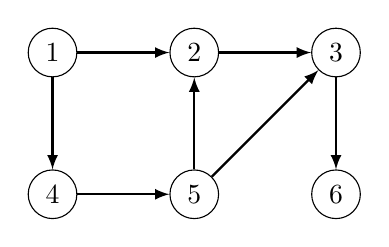
\begin{tikzpicture}[scale=0.9]
\node[draw, circle] (1) at (1,5) {$1$};
\node[draw, circle] (2) at (3,5) {$2$};
\node[draw, circle] (3) at (5,5) {$3$};
\node[draw, circle] (4) at (1,3) {$4$};
\node[draw, circle] (5) at (3,3) {$5$};
\node[draw, circle] (6) at (5,3) {$6$};

\path[draw,thick,->,>=latex] (1) -- (2);
\path[draw,thick,->,>=latex] (2) -- (3);
\path[draw,thick,->,>=latex] (1) -- (4);
\path[draw,thick,->,>=latex] (4) -- (5);
\path[draw,thick,->,>=latex] (5) -- (2);
\path[draw,thick,->,>=latex] (5) -- (3);
\path[draw,thick,->,>=latex] (3) -- (6);
\end{tikzpicture}
\end{center}
这样的路径共有三条：
\begin{itemize}
\item $1 \rightarrow 2 \rightarrow 3 \rightarrow 6$
\item $1 \rightarrow 4 \rightarrow 5 \rightarrow 2 \rightarrow 3 \rightarrow 6$
\item $1 \rightarrow 4 \rightarrow 5 \rightarrow 3 \rightarrow 6$
\end{itemize}

令 $\texttt{paths}(x)$ 表示从节点1到节点 $x$ 的路径数量。
作为基础情形，$\texttt{paths}(1)=1$。
然后，要计算 $\texttt{paths}(x)$ 的其他值，
我们可以使用递推公式
\[\texttt{paths}(x) = \texttt{paths}(a_1)+\texttt{paths}(a_2)+\cdots+\texttt{paths}(a_k)\]
其中 $a_1,a_2,\ldots,a_k$ 是有边指向 $x$ 的节点。
由于图是无环的，$\texttt{paths}(x)$ 的值
可以按拓扑排序的顺序计算。
上图的一个拓扑排序如下：
\begin{center}
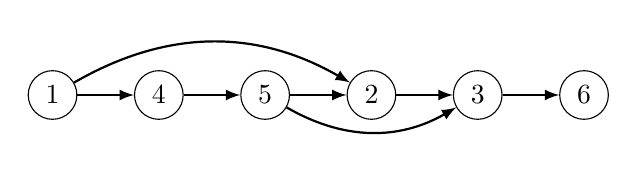
\begin{tikzpicture}[scale=0.9]
\node[draw, circle] (1) at (0,0) {$1$};
\node[draw, circle] (2) at (4.5,0) {$2$};
\node[draw, circle] (3) at (6,0) {$3$};
\node[draw, circle] (4) at (1.5,0) {$4$};
\node[draw, circle] (5) at (3,0) {$5$};
\node[draw, circle] (6) at (7.5,0) {$6$};

\path[draw,thick,->,>=latex] (1) edge [bend left=30] (2);
\path[draw,thick,->,>=latex] (2) -- (3);
\path[draw,thick,->,>=latex] (1) -- (4);
\path[draw,thick,->,>=latex] (4) -- (5);
\path[draw,thick,->,>=latex] (5) -- (2);
\path[draw,thick,->,>=latex] (5) edge [bend right=30] (3);
\path[draw,thick,->,>=latex] (3) -- (6);
\end{tikzpicture}
\end{center}
因此，路径数量如下：
\begin{center}
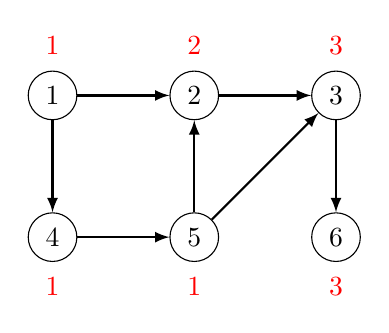
\begin{tikzpicture}[scale=0.9]
\node[draw, circle] (1) at (1,5) {$1$};
\node[draw, circle] (2) at (3,5) {$2$};
\node[draw, circle] (3) at (5,5) {$3$};
\node[draw, circle] (4) at (1,3) {$4$};
\node[draw, circle] (5) at (3,3) {$5$};
\node[draw, circle] (6) at (5,3) {$6$};

\path[draw,thick,->,>=latex] (1) -- (2);
\path[draw,thick,->,>=latex] (2) -- (3);
\path[draw,thick,->,>=latex] (1) -- (4);
\path[draw,thick,->,>=latex] (4) -- (5);
\path[draw,thick,->,>=latex] (5) -- (2);
\path[draw,thick,->,>=latex] (5) -- (3);
\path[draw,thick,->,>=latex] (3) -- (6);

\node[color=red] at (1,2.3) {$1$};
\node[color=red] at (3,2.3) {$1$};
\node[color=red] at (5,2.3) {$3$};
\node[color=red] at (1,5.7) {$1$};
\node[color=red] at (3,5.7) {$2$};
\node[color=red] at (5,5.7) {$3$};
\end{tikzpicture}
\end{center}

例如，要计算 $\texttt{paths}(3)$ 的值，
我们可以使用公式 $\texttt{paths}(2)+\texttt{paths}(5)$，
因为节点2和5有边指向节点3。
由于 $\texttt{paths}(2)=2$ 且 $\texttt{paths}(5)=1$，我们得出 $\texttt{paths}(3)=3$。

\subsubsection{扩展Dijkstra算法}

\index{Dijkstra算法}

Dijkstra算法的一个副产品是一个有向无环图，
它指示了原图中每个节点从起始节点出发的最短路径的可能到达方式。
可以对该图应用动态规划。
例如，在以下图中
\begin{center}
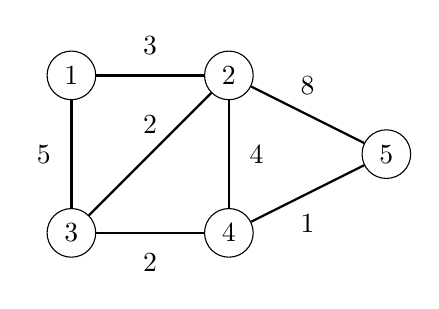
\begin{tikzpicture}
\node[draw, circle] (1) at (0,0) {$1$};
\node[draw, circle] (2) at (2,0) {$2$};
\node[draw, circle] (3) at (0,-2) {$3$};
\node[draw, circle] (4) at (2,-2) {$4$};
\node[draw, circle] (5) at (4,-1) {$5$};

\path[draw,thick,-] (1) -- node[font=\small,label=above:3] {} (2);
\path[draw,thick,-] (1) -- node[font=\small,label=left:5] {} (3);
\path[draw,thick,-] (2) -- node[font=\small,label=right:4] {} (4);
\path[draw,thick,-] (2) -- node[font=\small,label=above:8] {} (5);
\path[draw,thick,-] (3) -- node[font=\small,label=below:2] {} (4);
\path[draw,thick,-] (4) -- node[font=\small,label=below:1] {} (5);
\path[draw,thick,-] (2) -- node[font=\small,label=above:2] {} (3);
\end{tikzpicture}
\end{center}
从节点1出发的最短路径可能使用以下边：
\begin{center}
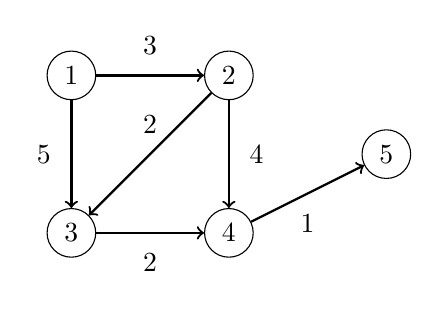
\begin{tikzpicture}
\node[draw, circle] (1) at (0,0) {$1$};
\node[draw, circle] (2) at (2,0) {$2$};
\node[draw, circle] (3) at (0,-2) {$3$};
\node[draw, circle] (4) at (2,-2) {$4$};
\node[draw, circle] (5) at (4,-1) {$5$};

\path[draw,thick,->] (1) -- node[font=\small,label=above:3] {} (2);
\path[draw,thick,->] (1) -- node[font=\small,label=left:5] {} (3);
\path[draw,thick,->] (2) -- node[font=\small,label=right:4] {} (4);
\path[draw,thick,->] (3) -- node[font=\small,label=below:2] {} (4);
\path[draw,thick,->] (4) -- node[font=\small,label=below:1] {} (5);
\path[draw,thick,->] (2) -- node[font=\small,label=above:2] {} (3);
\end{tikzpicture}
\end{center}

现在，我们可以使用动态规划计算从节点1到节点5的最短路径数量：
\begin{center}
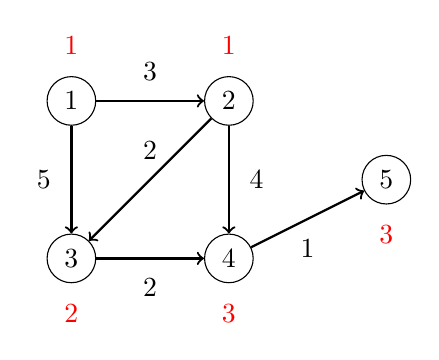
\begin{tikzpicture}
\node[draw, circle] (1) at (0,0) {$1$};
\node[draw, circle] (2) at (2,0) {$2$};
\node[draw, circle] (3) at (0,-2) {$3$};
\node[draw, circle] (4) at (2,-2) {$4$};
\node[draw, circle] (5) at (4,-1) {$5$};

\path[draw,thick,->] (1) -- node[font=\small,label=above:3] {} (2);
\path[draw,thick,->] (1) -- node[font=\small,label=left:5] {} (3);
\path[draw,thick,->] (2) -- node[font=\small,label=right:4] {} (4);
\path[draw,thick,->] (3) -- node[font=\small,label=below:2] {} (4);
\path[draw,thick,->] (4) -- node[font=\small,label=below:1] {} (5);
\path[draw,thick,->] (2) -- node[font=\small,label=above:2] {} (3);

\node[color=red] at (0,0.7) {$1$};
\node[color=red] at (2,0.7) {$1$};
\node[color=red] at (0,-2.7) {$2$};
\node[color=red] at (2,-2.7) {$3$};
\node[color=red] at (4,-1.7) {$3$};
\end{tikzpicture}
\end{center}

\subsubsection{将问题表示为图}

实际上，任何动态规划问题都可以表示为有向无环图。
在这样的图中，每个节点对应一个动态规划状态，
边指示状态之间的依赖关系。

例如，考虑使用硬币
$\{c_1,c_2,\ldots,c_k\}$
凑成金额 $n$ 的问题。
在这个问题中，我们可以构造一个图，其中每个节点对应一个金额，
边表示硬币的选择方式。
例如，对于硬币 $\{1,3,4\}$ 和 $n=6$，
图如下：
\begin{center}
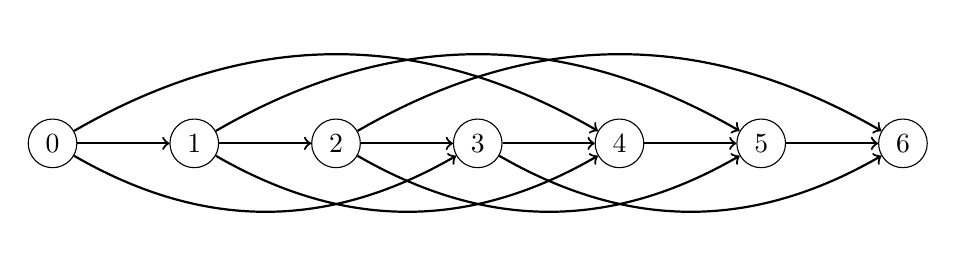
\begin{tikzpicture}[scale=0.9]
\node[draw, circle] (0) at (0,0) {$0$};
\node[draw, circle] (1) at (2,0) {$1$};
\node[draw, circle] (2) at (4,0) {$2$};
\node[draw, circle] (3) at (6,0) {$3$};
\node[draw, circle] (4) at (8,0) {$4$};
\node[draw, circle] (5) at (10,0) {$5$};
\node[draw, circle] (6) at (12,0) {$6$};

\path[draw,thick,->] (0) -- (1);
\path[draw,thick,->] (1) -- (2);
\path[draw,thick,->] (2) -- (3);
\path[draw,thick,->] (3) -- (4);
\path[draw,thick,->] (4) -- (5);
\path[draw,thick,->] (5) -- (6);

\path[draw,thick,->] (0) edge [bend right=30] (3);
\path[draw,thick,->] (1) edge [bend right=30] (4);
\path[draw,thick,->] (2) edge [bend right=30] (5);
\path[draw,thick,->] (3) edge [bend right=30] (6);

\path[draw,thick,->] (0) edge [bend left=30] (4);
\path[draw,thick,->] (1) edge [bend left=30] (5);
\path[draw,thick,->] (2) edge [bend left=30] (6);
\end{tikzpicture}
\end{center}

使用这种表示，
从节点0到节点 $n$ 的最短路径对应于使用最少硬币数的解，
而从节点0到节点 $n$ 的路径总数等于解的总数。

\section{后继路径}

\index{后继图}
\index{函数图}

在本章余下部分，
我们将关注\key{后继图}。
在这些图中，每个节点的出度为1，即每个节点恰好有一条边出发。
后继图由一个或多个连通分量组成，每个连通分量包含一个环和一些通向该环的路径。

后继图有时被称为
\key{函数图}。
这是因为任何后继图都对应一个定义图边的函数。
函数的参数是图中的一个节点，
函数返回该节点的后继。

例如，以下函数
\begin{center}
\begin{tabular}{r|rrrrrrrrr}
$x$ & 1 & 2 & 3 & 4 & 5 & 6 & 7 & 8 & 9 \\
\hline
$\texttt{succ}(x)$ & 3 & 5 & 7 & 6 & 2 & 2 & 1 & 6 & 3 \\
\end{tabular}
\end{center}
定义了以下图：
\begin{center}
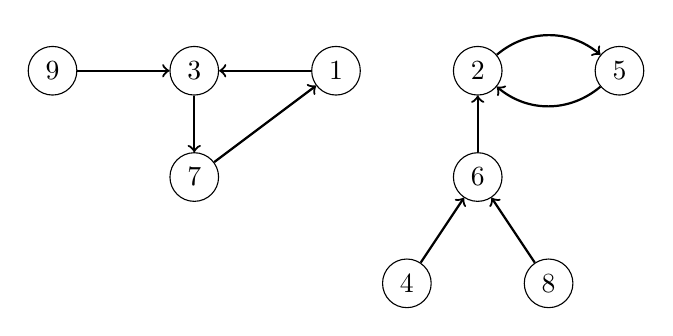
\begin{tikzpicture}[scale=0.9]
\node[draw, circle] (1) at (0,0) {$1$};
\node[draw, circle] (2) at (2,0) {$2$};
\node[draw, circle] (3) at (-2,0) {$3$};
\node[draw, circle] (4) at (1,-3) {$4$};
\node[draw, circle] (5) at (4,0) {$5$};
\node[draw, circle] (6) at (2,-1.5) {$6$};
\node[draw, circle] (7) at (-2,-1.5) {$7$};
\node[draw, circle] (8) at (3,-3) {$8$};
\node[draw, circle] (9) at (-4,0) {$9$};

\path[draw,thick,->] (1) -- (3);
\path[draw,thick,->] (2)  edge [bend left=40] (5);
\path[draw,thick,->] (3) -- (7);
\path[draw,thick,->] (4) -- (6);
\path[draw,thick,->] (5)  edge [bend left=40] (2);
\path[draw,thick,->] (6) -- (2);
\path[draw,thick,->] (7) -- (1);
\path[draw,thick,->] (8) -- (6);
\path[draw,thick,->] (9) -- (3);
\end{tikzpicture}
\end{center}

由于后继图的每个节点都有唯一后继，我们还可以定义函数 $\texttt{succ}(x,k)$，
它返回从节点 $x$ 出发向前走 $k$ 步后到达的节点。
例如，在上图中 $\texttt{succ}(4,6)=2$，
因为从节点4出发走6步将到达节点2：

\begin{center}
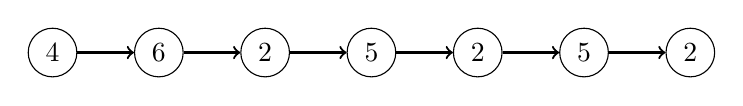
\begin{tikzpicture}[scale=0.9]
\node[draw, circle] (1) at (0,0) {$4$};
\node[draw, circle] (2) at (1.5,0) {$6$};
\node[draw, circle] (3) at (3,0) {$2$};
\node[draw, circle] (4) at (4.5,0) {$5$};
\node[draw, circle] (5) at (6,0) {$2$};
\node[draw, circle] (6) at (7.5,0) {$5$};
\node[draw, circle] (7) at (9,0) {$2$};

\path[draw,thick,->] (1) -- (2);
\path[draw,thick,->] (2) -- (3);
\path[draw,thick,->] (3) -- (4);
\path[draw,thick,->] (4) -- (5);
\path[draw,thick,->] (5) -- (6);
\path[draw,thick,->] (6) -- (7);
\end{tikzpicture}
\end{center}

计算 $\texttt{succ}(x,k)$ 值的一种直接方法是从节点 $x$ 出发走 $k$ 步，这需要 $O(k)$ 时间。
然而，通过预处理，任何 $\texttt{succ}(x,k)$ 的值可以在仅 $O(\log k)$ 时间内计算出来。

基本思想是预先计算所有 $k$ 为2的幂且不超过 $u$ 的 $\texttt{succ}(x,k)$ 值，其中 $u$ 是我们可能走的最大步数。
这可以高效完成，因为我们可以使用以下递推：

\begin{equation*}
    \texttt{succ}(x,k) = \begin{cases}
               \texttt{succ}(x)              & k = 1\\
               \texttt{succ}(\texttt{succ}(x,k/2),k/2)   & k > 1\\
           \end{cases}
\end{equation*}

预处理这些值需要 $O(n \log u)$ 时间，
因为每个节点需要计算 $O(\log u)$ 个值。
在上图中，前几个值如下：

\begin{center}
\begin{tabular}{r|rrrrrrrrr}
$x$ & 1 & 2 & 3 & 4 & 5 & 6 & 7 & 8 & 9 \\
\hline
$\texttt{succ}(x,1)$ & 3 & 5 & 7 & 6 & 2 & 2 & 1 & 6 & 3 \\
$\texttt{succ}(x,2)$ & 7 & 2 & 1 & 2 & 5 & 5 & 3 & 2 & 7 \\
$\texttt{succ}(x,4)$ & 3 & 2 & 7 & 2 & 5 & 5 & 1 & 2 & 3 \\
$\texttt{succ}(x,8)$ & 7 & 2 & 1 & 2 & 5 & 5 & 3 & 2 & 7 \\
$\cdots$ \\
\end{tabular}
\end{center}

此后，任何 $\texttt{succ}(x,k)$ 的值都可以通过将步数 $k$ 表示为2的幂之和来计算。
例如，如果我们想计算 $\texttt{succ}(x,11)$ 的值，
首先将 $11$ 表示为 $11=8+2+1$。
利用这个表示，
\[\texttt{succ}(x,11)=\texttt{succ}(\texttt{succ}(\texttt{succ}(x,8),2),1).\]
例如，在上一个图中
\[\texttt{succ}(4,11)=\texttt{succ}(\texttt{succ}(\texttt{succ}(4,8),2),1)=5.\]

这样的表示总是由 $O(\log k)$ 部分组成，因此计算 $\texttt{succ}(x,k)$ 的值需要 $O(\log k)$ 时间。

\section{环检测}

\index{环}
\index{环检测}

考虑一个只包含一条以环结尾的路径的后继图。
我们可以提出以下问题：如果我们从起始节点开始行走，
环中的第一个节点是什么，环包含多少个节点？

例如，在以下图中

\begin{center}
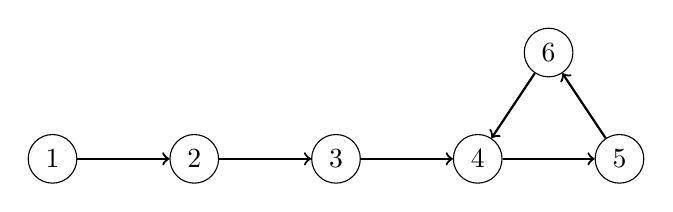
\begin{tikzpicture}[scale=0.9]
\node[draw, circle] (5) at (0,0) {$5$};
\node[draw, circle] (4) at (-2,0) {$4$};
\node[draw, circle] (6) at (-1,1.5) {$6$};
\node[draw, circle] (3) at (-4,0) {$3$};
\node[draw, circle] (2) at (-6,0) {$2$};
\node[draw, circle] (1) at (-8,0) {$1$};

\path[draw,thick,->] (1) -- (2);
\path[draw,thick,->] (2) -- (3);
\path[draw,thick,->] (3) -- (4);
\path[draw,thick,->] (4) -- (5);
\path[draw,thick,->] (5) -- (6);
\path[draw,thick,->] (6) -- (4);
\end{tikzpicture}
\end{center}
我们从节点1开始行走，
环中的第一个节点是节点4，环由三个节点组成（4、5和6）。

检测环的一种简单方法是在图中行走并记录所有已访问的节点。一旦某个节点被第二次访问，
我们就可以得出结论该节点是环中的第一个节点。
这种方法的时间复杂度为 $O(n)$，空间复杂度也为 $O(n)$。

然而，还有更好的环检测算法。
这些算法的时间复杂度仍然是 $O(n)$，但仅使用 $O(1)$ 的空间。
当 $n$ 较大时，这是一个重要的改进。
接下来我们将讨论Floyd算法，该算法具有这些性质。

\subsubsection{Floyd算法}

\index{Floyd算法}

\key{Floyd算法}\footnote{该算法的思想在 \cite{knu982} 中被提及，并归功于R. W. Floyd；然而，目前尚不清楚Floyd是否真的发现了该算法。} 使用两个指针 $a$ 和 $b$ 在图中向前行走。
两个指针都从图中的起始节点 $x$ 开始。
然后，每一轮中，指针 $a$ 向前走一步，指针 $b$ 向前走两步。
这个过程持续进行直到两个指针相遇：
\begin{lstlisting}
a = succ(x);
b = succ(succ(x));
while (a != b) {
    a = succ(a);
    b = succ(succ(b));
}
\end{lstlisting}

此时，指针 $a$ 走了 $k$ 步，
指针 $b$ 走了 $2k$ 步，
因此环的长度是 $k$ 的因子。
因此，要找到环中的第一个节点，可以将指针 $a$ 移回节点 $x$，
然后逐步推进两个指针直到它们再次相遇。
\begin{lstlisting}
a = x;
while (a != b) {
    a = succ(a);
    b = succ(b);
}
first = a;
\end{lstlisting}

此后，环的长度可以如下计算：
\begin{lstlisting}
b = succ(a);
length = 1;
while (a != b) {
    b = succ(b);
    length++;
}
\end{lstlisting}
